Le début de mon stage s'est focalisé sur le développement d'interfaces. Plus spécifiquement, j'ai travaillé sur l'affichage des 'régions d'image', anciennement appelées 'annotations' (correspondant aux extractions), ainsi que des vectorisations associées. J'ai pu ainsi approfondir ma compréhension du \textit{framework} Django en me familiarisant avec le processus de création de vues personnalisées. Néanmoins, ces vues ont été amenées à évoluer au fil des développements effectués par l'équipe de développeur.ses du projet. En effet, le principe de la 'vue' est d'interfacer le rendu graphique et le modèle de données, et ce dernier a été amené à évoluer au cours de mon stage. Cette annexe présente les développements effectués et certaines de leurs évolutions. 

\section{\texttt{views.py} pour traiter la logique des requêtes}

Ce fichier contient les fonctions ou classes appelées 'vues' qui traitent les requêtes \http envoyées par l'utilisateur.rice. Chaque vue correspond généralement à une fonctionnalité spécifique de l'application. Elle récupère des données, souvent formatées grâce à des méthodes de classes, elle peut les traiter, et retourne une réponse \http (comme une page \html, un fichier \json, etc.).

Lorsque l'utilisateur.rice visite une \URL spécifique, Django appelle la vue correspondante pour générer la réponse.

Par exemple, l'\URL qui affiche les résultats de l'extraction peut appeler la fonction suivante~:

\begin{lstlisting}[language=python, frame=single, breaklines=true, caption={Vue pour l'affichage des extraction en \enquote{dump}.}]
# /app/webapp/views.py

@login_required(login_url=f"/{APP_NAME}-admin/login/")
def show_all_annotations(request, anno_ref):
    passed, anno = check_ref(anno_ref, "Annotation")
    if not passed:
        return JsonResponse(anno)

    if not ENV("DEBUG"):
        credentials(f"{SAS_APP_URL}/", ENV("SAS_USERNAME"), ENV("SAS_PASSWORD"))

    _, all_annos = formatted_annotations(anno)
    all_crops = [
        (canvas_nb, coord, img_file)
        for canvas_nb, coord, img_file in all_annos
        if coord
    ]

    paginator = Paginator(all_crops, 50)
    try:
        page_annos = paginator.page(request.GET.get("page"))
    except PageNotAnInteger:
        page_annos = paginator.page(1)
    except EmptyPage:
        page_annos = paginator.page(paginator.num_pages)

    return render(
        request,
        "show_crops.html",
        context={
            "anno": anno,
            "page_annos": page_annos,
            "all_crops": all_crops,
            "url_manifest": anno.gen_manifest_url(version=MANIFEST_V2),
            "anno_ref": anno_ref,
        },
    )
\end{lstlisting}

La fonction envoie au \textit{template} des métadonnées, ainsi que les coordonnées des annotations, pour chaque page annotée. Les régions d'images seront appelées dynamiquement dans le \textit{template} grâce à la reconstruction à la volée des \URLs \iiif. 

L'action utilisateur.rice pour exporter l'ensemble des \textit{crops} de diagramme d'un témoin en \jpeg et sous forme de \textsc{zip} appelle la vue suivante~: 

\begin{lstlisting}[language=python, frame=single, breaklines=true, caption={Vue pour l'export de l'ensemble des diagrammes du témoin affiché.}]
@login_required(login_url=f"/{APP_NAME}-admin/login/")
def export_all_crops(request, anno_ref):
    passed, anno = check_ref(anno_ref, "Annotation")
    if not passed:
        return JsonResponse(anno)

    if not ENV("DEBUG"):
        credentials(f"{SAS_APP_URL}/", ENV("SAS_USERNAME"), ENV("SAS_PASSWORD"))

    urls_list = []

    _, all_annos = formatted_annotations(anno)
    all_crops = [
        (canvas_nb, coord, img_file)
        for canvas_nb, coord, img_file in all_annos
        if coord
    ]

    for canvas_nb, coord, img_file in all_crops:
        urls_list.extend(gen_iiif_url(img_file, 2, f"{c[0]}/full/0") for c in coord)

    return zip_img(urls_list)
\end{lstlisting}

Enfin, une vue a été créée pour exporter uniquement les diagrammes sélectionnés. La liste est créée côté navigateur grâce à du JavaScript.  

\begin{lstlisting}[language=python, frame=single, breaklines=true, caption={Vue pour l'export d'une liste de diagrammes.}]
@login_required(login_url=f"/{APP_NAME}-admin/login/")
def export_selected_crops(request):

    urls_list = json.loads(request.POST.get("listeURL"))

    return zip_img(urls_list)
\end{lstlisting}

Les vues font appel à de nombreuses autres fonctions utilitaires ou méthodes de classe, par exemple \texttt{formatted\_annotations}, situé dans un fichier du dossier utilitaire dédié aux annotations \iiif (\texttt{app/webapp/utils/iiif/annotation.py}). Elle génère une liste structurée d'annotations. Pour chaque image, dans les données fournies par l'entité \textit{Regions}, la fonction récupère les annotations associées. Si des annotations existent pour une image donnée, elle extrait pour chacune ses coordonnées et son identifiant. 

\section{\texttt{url.py} pour le routage des \URLs}

Ce fichier définit les correspondances entre les \URLs entrées par l'utilisateur.rice et les vues dans \texttt{views.py}. Il lie les requêtes \URL spécifiques aux fonctions appropriées. Lorsqu'une requête est faite par l'utilisateur.rice, Django utilise \texttt{urls.py} pour déterminer quelle vue doit être exécutée en fonction de l'\URL.

Indexation des vues dans le fichier \texttt{urls.py}~:

\begin{lstlisting}[language=python, frame=single, breaklines=true, caption={Contenu du ficher \texttt{urls.py}~: import des \texttt{views}.}]
#/app/config/urls.py
from app.webapp.views import (
...
show_all_annotations,
export_all_crops,
export_selected_crops,
...
)
\end{lstlisting}

\begin{lstlisting}[language=python, frame=single, breaklines=true, caption={Contenu du ficher \texttt{urls.py}~: routage des fonctions et des \URLs.}]
urlpatterns = [
    ...
    path(
        f"{APP_NAME}/<str:anno_ref>/show-all-annotations",
        show_all_annotations,
        name="show-all-annotations",
    ),

    path(
        f"{APP_NAME}/export-crops/<str:anno_ref>",
        export_all_crops,
        name="export-crops",
    ),

    path(
        f"{APP_NAME}/export-selected-crops",
        export_selected_crops,
        name="export-selected-crops",
    ),

    path(
        f"{APP_NAME}/<str:anno_ref>/show-vectorization",
        show_vectorization,
        name="show-vectorization",
    ),
    ...
]
\end{lstlisting}

\section{Les \emph{templates}}

Les \textit{templates} sont des fichiers \html (avec éventuellement des balises Django) qui définissent la présentation de la réponse envoyée à l'utilisateur.rice. Ils permettent de séparer la logique de l'application (dans les vues) de la présentation (dans les \textit{templates}).

\begin{lstlisting}[language=HTML5, frame=single, breaklines=true, caption={Template \html pour l'affichage des crops de diagrammes.}]
{#/app/webapp/templates/show_crops.html#}


    <div class="toolbar">
        <div class="title">
            <b>{{ anno|capfirst }}</b>
        </div>

        <div style="display: flex; flex-direction: row;">
            <a href="">
                <button class="export-button" type="submit">
                    <i class="fa-regular fa-file-zipper"></i>&nbsp;
                    
                        Download all
                    
                        Télécharger toutes les
                    
                    annotations
                </button>
            </a>

            <form id="export" action="" method="post">
                
                <input type="hidden" id="listeURL" name="listeURL" value="">
                <button class="export-button" type="submit">
                    <i class="fa-regular fa-file-zipper"></i>&nbsp;
                    
                        Download selected annotations
                    
                        Télécharger les annotations sélectionnées
                    
                </button>
            </form>

            
                <a href="" target="_blank">
                    <button class="edit-button" type="submit">
                        <i class="fa fa-pencil"></i>&nbsp;
                        
                            Edit
                        
                            Éditer les
                        
                        annotations
                    </button>
                </a>
            
        </div>
    </div>




<div class="tabs-crops">
    <div class="row">
        <div class="tab-buttons">
            <button class="btn-change active-tab">
                Page view
            
                Vue page
            
            </button>
            <button class="btn-change">
                Dump view
            
                Vue générale
            
            </button>
        </div>
    </div>

    <div class="tab-bodies">
        <div class="row" style="display:block;">
            <div class="column">
                <table class="anno-table" style="margin-top: 0em;">
                    
                        <tr class="anno-row">
                            <td class="anno-td page-col">
                                <a href="{{ img_file|img_to_iiif}}" target="_blank">
                                    <img class="page-preview" src="{{ img_file|img_to_iiif:"full/350,/0" }}" alt="Click to see real size image">
                                </a>
                                <h3><a href="{{ img_file|img_to_iiif }}" target="_blank">Page {{ canvas_nb }}</a></h3>
                            </td>
                            <td class="anno-td anno-col">
                                
                                    <div id="ill_{{ id }}" class="anno-div">
                                        
                                            <a href="{{ img_file|img_to_iiif:region_full }}" target="_blank">
                                                <img src="{{ img_file|img_to_iiif:region }}" alt="scan preview">
                                            </a>
                                            <br>
                                            <input id="bbox_{{ id }}" type="checkbox" name="crop_checkbox" value="{{ img_file|img_to_iiif:region_full }}" onchange="updateSelectedImageURLs()">
                                            <label for="bbox_{{ id }}">
                                                SelectSélectionner
                                            </label>
                                        
                                    </div>
                                
                            </td>
                        </tr>
                    
                </table>
                
            </div>
        </div>

        <div style="display:none;">
            <div class="grid-container" style="margin-top: .5em;">
                
                    
                        
                            <div class="grid-item">
                                <a href="{{ img_file|img_to_iiif:region_full }}" target="_blank">
                                    <img src="{{ img_file|img_to_iiif:region }}" alt="scan preview">
                                </a>
                                <h3><a href="{{ img_file|img_to_iiif }}" target="_blank">Page {{ canvas_nb }}</a></h3>
                                <input id="bbox_{{ id }}" type="checkbox" name="crop_checkbox" value="{{ img_file|img_to_iiif:region_full }}" onchange="updateSelectedImageURLs()">
                                <label for="bbox_{{ id }}">
                                    SelectSélectionner
                                </label>
                            </div>
                        
                    
                
            </div>
        </div>
    </div>
</div>

<script>
    var checkboxes = document.querySelectorAll('input[name="crop_checkbox"]');
    var selectedImageURLs = [];
    // Fonction pour mettre à jour la liste des URL sélectionnées
    function updateSelectedImageURLs() {
        // Réinitialiser la liste des URL sélectionnées
        selectedImageURLs = [];

        // Parcourir toutes les cases à cocher
        checkboxes.forEach(function(checkbox) {
            // Vérifier si la case est cochée
            if (checkbox.checked) {
                // Récupérez l'URL de l'image à partir de la value de la case cochée
                var imageURL = checkbox.value;
                // Ajouter l'URL de l'image à la liste des URL sélectionnées
                selectedImageURLs.push(imageURL);
                }
            }
        );
        // Afficher la liste des URLs sélectionnées
        console.log(selectedImageURLs);
        var jsonString = JSON.stringify(selectedImageURLs);

        // liste => hidden input
        document.getElementById("listeURL").value = jsonString;
        // Vérifier si la valeur du champ est correcte
        console.log(document.getElementById("listeURL").value);
    };

    Array.from(document.querySelectorAll('.tabs-crops')).forEach((tab_container, TabID) => {
        const registers = tab_container.querySelector('.tab-buttons');
        const bodies = tab_container.querySelector('.tab-bodies');

        Array.from(registers.children).forEach((el, i) => {
          el.setAttribute('aria-controls', `${TabID}_${i}`)
          bodies.children[i]?.setAttribute('id', `${TabID}_${i}`)

          el.addEventListener('click', (ev) => {
            let activeRegister = registers.querySelector('.active-tab');
            activeRegister.classList.remove('active-tab')
            activeRegister = el;
            activeRegister.classList.add('active-tab')
            changeBody(registers, bodies, activeRegister)
          })
      })
    })

    function changeBody(registers, bodies, activeRegister) {
        selectedImageURLs = [];

        checkboxes.forEach(function(checkbox) {
        checkbox.checked = false;
        });

        Array.from(registers.children).forEach((el, i) => {

            if (bodies.children[i]) {
                bodies.children[i].style.display = el == activeRegister~? 'block'~: 'none'
            }

            el.setAttribute('aria-expanded', el == activeRegister~? 'true'~: 'false')
        })
    }
</script>


\end{lstlisting}

Ce qui donne deux affichages possibles pour les extractions~: 

          \begin{figure}[H]
          \begin{center}
          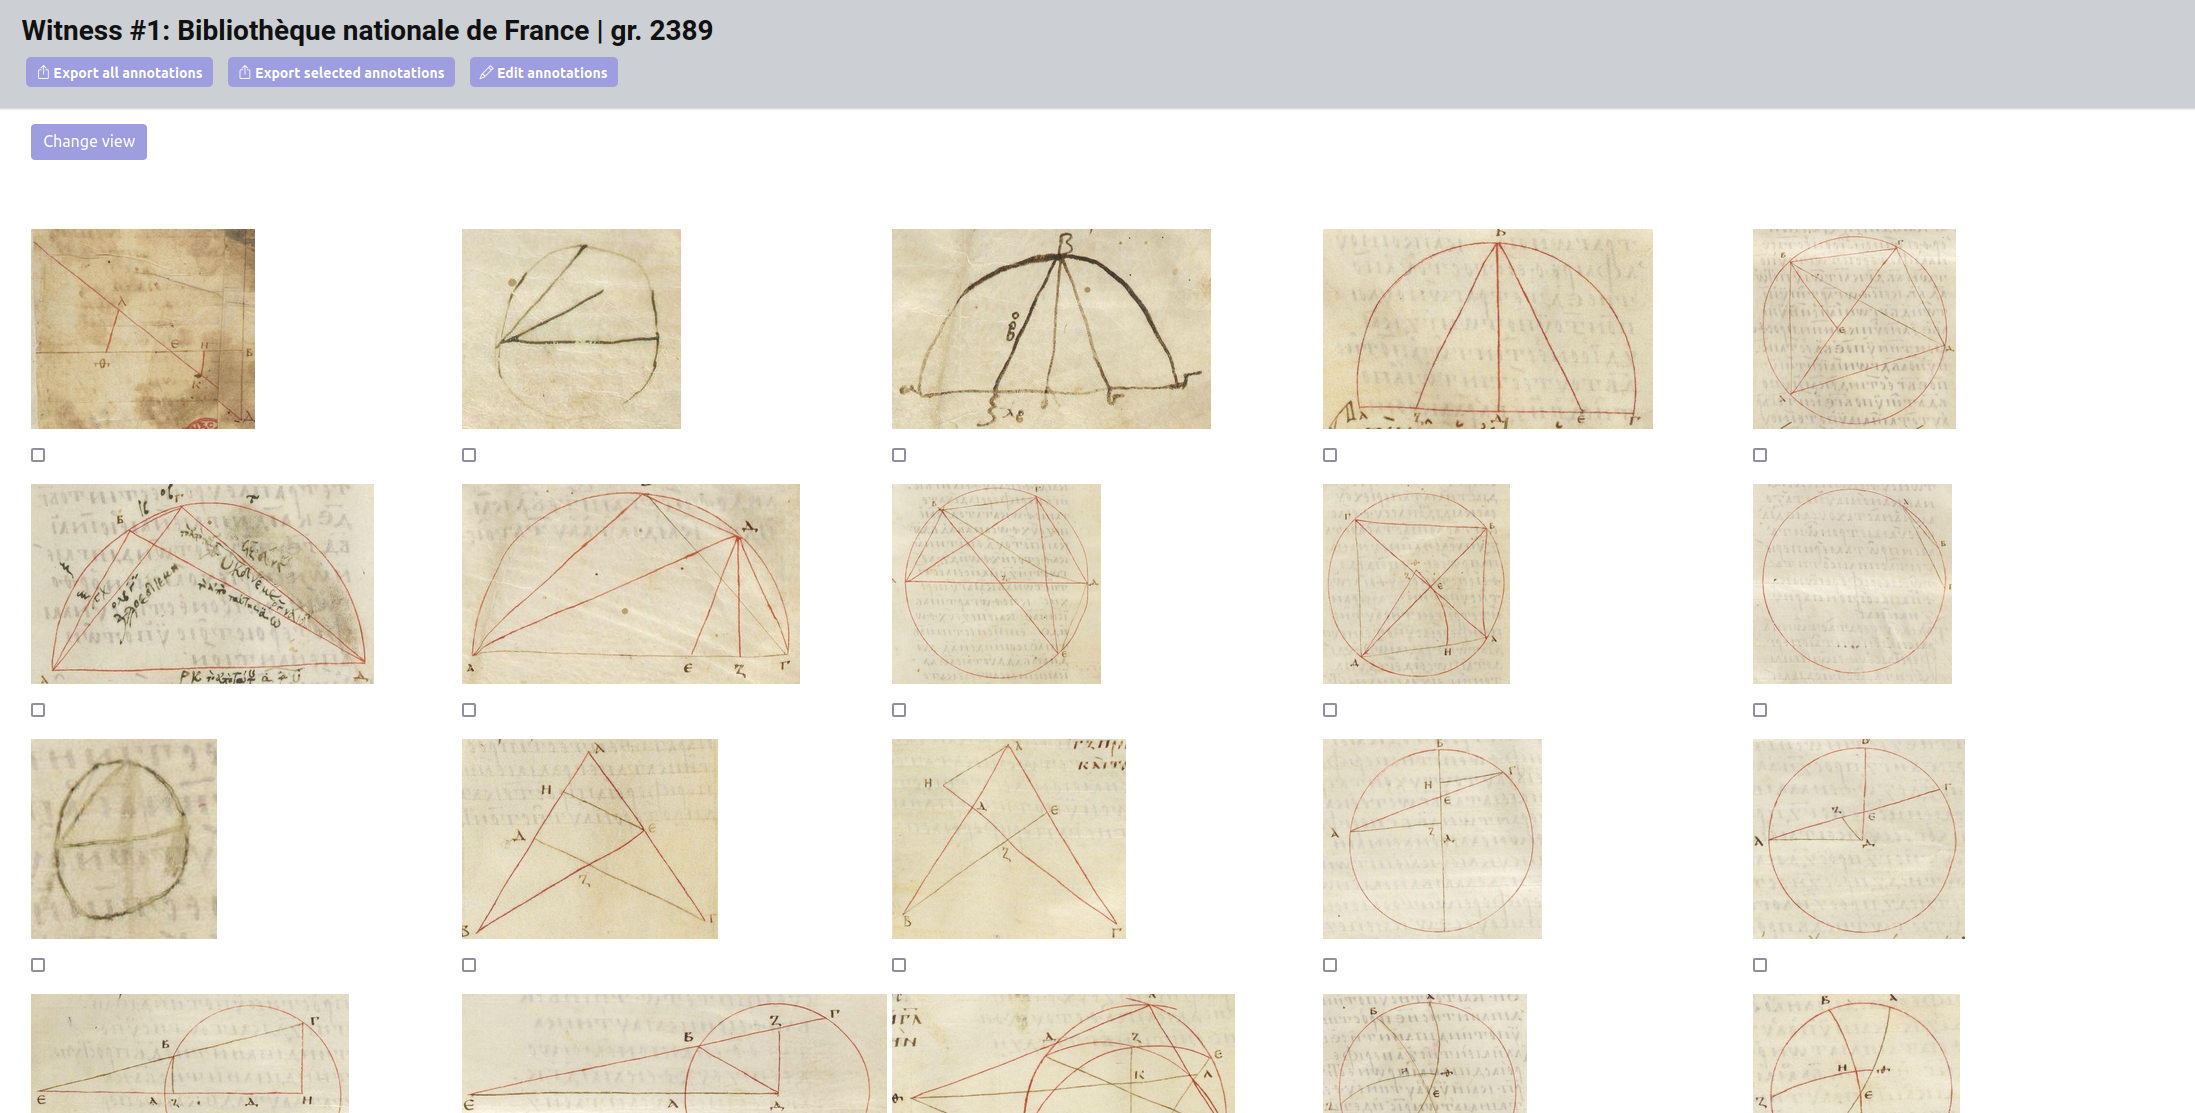
\includegraphics[height=7cm]{figues/vue_dump.png}
          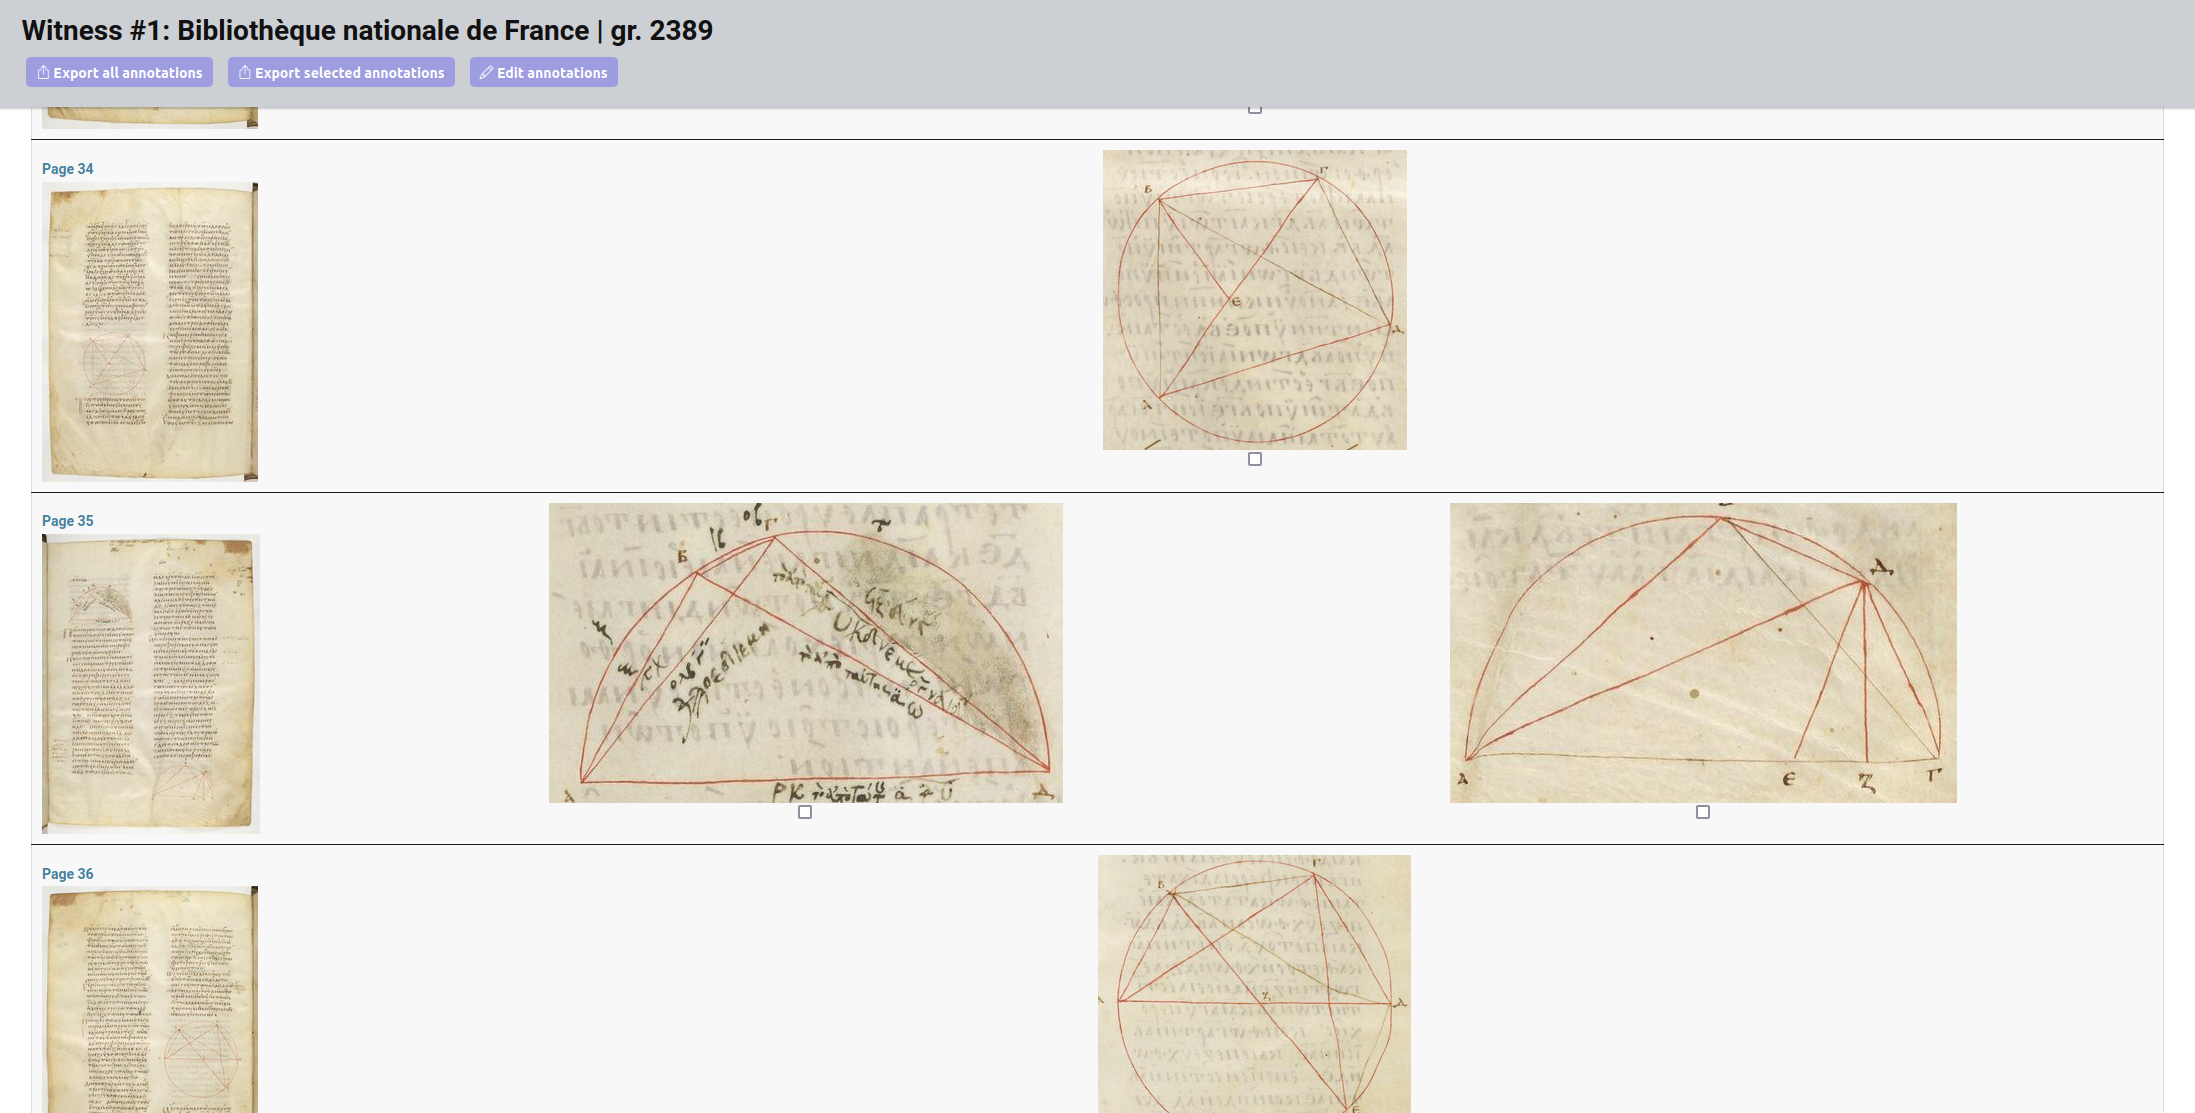
\includegraphics[height=7cm]{figues/vue_contexte.png}
          \end{center}
          \caption{Affichage des extractions, vue \emph{dump} et avec la page de manuscrit en regard.}
          \label{fig:old_interface_1} \end{figure}

Des vues similaires ont été créées pour afficher les résultats de la vectorisation. 

\section{Autres développements }

Vues pour l'export des \svgs et des images \jpeg~: 

\begin{lstlisting}[language=python, frame=single, breaklines=true, caption={Vue pour l'export de tous les \svgs et des images associées.}]

@login_required(login_url=f"/{APP_NAME}-admin/login/")
def export_all_images_and_svgs(request, anno_ref):
    passed, anno = check_ref(anno_ref, "Annotation")
    if not passed:
        return JsonResponse(anno)

    if not ENV("DEBUG"):
        credentials(f"{SAS_APP_URL}/", ENV("SAS_USERNAME"), ENV("SAS_PASSWORD"))

    urls_list = []
    path_list = []

    _, all_annos = formatted_annotations(anno)
    all_crops = [
        (canvas_nb, coord, img_file)
        for canvas_nb, coord, img_file in all_annos
        if coord
    ]

    for canvas_nb, coord, img_file in all_crops:
        urls_list.extend(gen_iiif_url(img_file, 2, f"{c[0]}/full/0") for c in coord)
        vecto_path = f"{img_file[:-4]}_{''.join(c[0] for c in coord)}.svg"
        # Vérifie si le chemin existe
        if os.path.exists(os.path.join(SVG_PATH, vecto_path)):
            path_list.append(vecto_path)

    return zip_images_and_files(urls_list, path_list)

\end{lstlisting}

\begin{lstlisting}[language=python, frame=single, breaklines=true, caption={Vue pour l'export des \svgs et des images \jpeg sélectionnés.}]
@login_required(login_url=f"/{APP_NAME}-admin/login/")
def export_selected_imgs_and_svgs(request):
    images_list = json.loads(request.POST.get("liste_images"))
    urls_list = []
    paths_list = []
    for element in images_list:
        if is_url(element):
            urls_list.append(element)
        else:
            paths_list.append(element)
    return zip_images_and_files(urls_list, paths_list)
\end{lstlisting}

Des fonctions utilitaires sont utiles pour assurer l'export~: 

\begin{lstlisting}[language=python, frame=single, breaklines=true, caption={Fonctions utilitaires pour compresser et télécharger les images.}]

def zip_img(img_list, zip_name=f"{APP_NAME}_export"):
    buffer = io.BytesIO()
    with zipfile.ZipFile(buffer, "w") as z:
        for img_path in img_list:
            img_name = f"{url_to_name(img_path)}.jpg"
            if urlparse(img_path).scheme == "":
                z.write(f"{IMG_PATH}/{img_name}", img_name)
            else:
                response = requests.get(img_path)
                if response.status_code == 200:
                    z.writestr(img_name, response.content)
                else:
                    log(f"[zip_img] Fail to download img: {img_path}")
                    pass

    response = HttpResponse(
        buffer.getvalue(), content_type="application/x-zip-compressed"
    )
    response["Content-Disposition"] = f"attachment; filename={zip_name}.zip"
    return response


def zip_files(filenames_contents, zip_name=f"{APP_NAME}_export"):
    # filenames_contents = [(filename1, content1), (filename2, content2), ...]
    buffer = io.BytesIO()
    with zipfile.ZipFile(buffer, "w") as z:
        for filename_content in filenames_contents:
            filename, content = filename_content
            z.writestr(filename, content)

    response = HttpResponse(
        buffer.getvalue(), content_type="application/x-zip-compressed"
    )
    response["Content-Disposition"] = f"attachment; filename={zip_name}.zip"
    return response


def zip_images_and_files(img_list, file_list, zip_name=f"{APP_NAME}_export"):
    buffer = io.BytesIO()
    with zipfile.ZipFile(buffer, "w") as z:
        # Ajouter des images à partir des URLs ou du répertoire local
        for img_path in img_list:
            img_name = f"{url_to_name(img_path)}.jpg"
            if urlparse(img_path).scheme == "":
                try:
                    z.write(f"{SVG_PATH}/{img_name}", img_name)
                except FileNotFoundError:
                    log(f"[zip_images_and_files] Local image not found: {img_path}")
            else:
                response = requests.get(img_path)
                if response.status_code == 200:
                    z.writestr(img_name, response.content)
                else:
                    log(f"[zip_images_and_files] Fail to download image: {img_path}")

        # Ajouter des fichiers à partir du répertoire mediafiles
        for file_path in file_list:
            try:
                with open(f"{SVG_PATH}/{file_path}", "rb") as f:
                    z.writestr(file_path, f.read())
            except FileNotFoundError:
                log(f"[zip_images_and_files] Local file not found: {file_path}")

    response = HttpResponse(
        buffer.getvalue(), content_type="application/x-zip-compressed"
    )
    response["Content-Disposition"] = f"attachment; filename={zip_name}.zip"
    return response

\end{lstlisting}

\textit{Template} pour afficher les \textit{crops} de diagrammes avec les vectorisations associées. Le \textit{template} et le rendu sont très similaire à ceux concernant l'affichage des diagrammes uniquement~: 

\begin{lstlisting}[language=HTML5, frame=single, breaklines=true, caption={Template \html pour afficher les extractions et leurs vectorisations.}]





{{ anno }}


    <div class="toolbar">
        <div class="title">
            <b>{{ anno|capfirst }}</b>
        </div>
        <div style="display: flex; flex-direction: row;">
            <a href="" target="_blank">
                <button class="export-button" type="submit">
                    <i class="fa-solid fa-eye"></i>
                    
                        Visualize all
                    
                        Voir toutes les
                    
                    annotations
                </button>
            </a>
            <a href="">
                <button class="export-button" type="submit">
                    <i class="fa-regular fa-file-zipper"></i>&nbsp;
                    
                        Download all
                    
                        Télécharger toutes les
                    
                    vectorisations
                </button>
            </a>

            <form id="export" action="" method="post">
                
                <input type="hidden" id="liste_images" name="liste_images" value="">
                <button class="export-button" type="submit">
                    <i class="fa-regular fa-file-zipper"></i>&nbsp;
                    
                        Download selected annotations
                    
                        Télécharger les vectorisations sélectionnées
                    
                </button>
            </form>
        </div>
    </div>




<div class="tabs-crops">
    <div class="row">
        <div class="tab-buttons">
            <button class="btn-change active-tab">
                Page view
            
                Vue page
            
            </button>
            <button class="btn-change">
                Dump view
            
                Vue générale
            
            </button>
        </div>
    </div>


<div class="tab-bodies">

    <div class="row" style="display:block;">
        <div class="column">
            <table class="anno-table" style="margin-top: 0em;">
                
                    <tr class="anno-row">
                        <td class="anno-td page-col">
                            <a href="{{ img_file|img_to_iiif}}" target="_blank">
                                <img class="page-preview" src="{{ img_file|img_to_iiif:"full/350,/0" }}" alt="Click to see real size image">
                            </a>
                            <h3><a href="{{ img_file|img_to_iiif }}" target="_blank">Page {{ canvas_nb }}</a></h3>
                        </td>
                        <td class="anno-td anno-col">
                            
                                <div id="ill_{{ id }}" class="anno-div grid-item" style=" display: flex; flex-wrap: wrap; justify-content: center;">
                                    
                                        <a href="{{ img_file|img_to_iiif:region_full }}" target="_blank">
                                            <img src="{{ img_file|img_to_iiif:region }}" alt="scan preview">
                                        </a>
                                        <img src="svg/{{ img_file|jpg_to_none }}_{{ coords }}.svg" class="img-fluid" alt="{{ img_file|jpg_to_none }}_{{ coords }}.svg">
                                        <a href="" target="_blank">VisualizeVisualiser</a>
                                        <br>
                                        <input type="checkbox" name="vecto_checkbox" value='["{{ img_file|jpg_to_none }}_{{ coords }}.svg", "{{ img_file|img_to_iiif:region }}"]' onchange="updateSelectedImageURLs()">
                                        <label for="checkbox">
                                            SelectSélectionner
                                        </label>
                                    
                                </div>
                            
                        </td>
                    </tr>
                
            </table>
            
        </div>
    </div>

    <div style="display: none;">
        <div style="margin-top: 5%;">
            <div class="grid-container">
                
                    
                        <div class="grid-item">
                            <div style="display: flex; flex-direction: row;">
                                
                                    <a href="{{ img_file|img_to_iiif:small }}" target="_blank">
                                        <img src="{{ img_file|img_to_iiif:small }}" class="img-fluid" alt="{{ img_file }}" style="margin-right: 10px;">
                                    </a>
                                            <img src="svg/{{ img_file|jpg_to_none }}_{{ coords }}.svg" class="img-fluid" alt="{{ img_file|jpg_to_none }}_{{ coords }}.svg">
                                            <a href="{ % url 'img-and-svg' img_file=img_file coords=coords %}" target="_blank">VisualizeVisualiser</a>
                                </a>
                                <input type="checkbox" name="vecto_checkbox" value='["{{ img_file|jpg_to_none }}_{{ coords }}.svg", "{{ img_file|img_to_iiif:small }}"]' onchange="updateSelectedImageURLs()">
                                
                            </div>
                            <h3><a href="{{ img_file|img_to_iiif }}" target="_blank">Page {{ canvas_nb }}</a></h3>
                        </div>
                    
                
            </div>
        </div>
    =</div>

</div>
</div>


<script>
    document.addEventListener('DOMContentLoaded', () => {
        const tabContainers = document.querySelectorAll('.tabs-crops');

        tabContainers.forEach((tabContainer, tabID) => {
            const registerButtons = tabContainer.querySelectorAll('.tab-buttons .btn-change');
            const tabBodies = tabContainer.querySelectorAll('.tab-bodies > div');

            registerButtons.forEach((button, index) => {
                button.setAttribute('aria-controls', `${tabID}_${index}`);
                if (tabBodies[index]) {
                    tabBodies[index].setAttribute('id', `${tabID}_${index}`);
                }

                button.addEventListener('click', () => {
                    setActiveTab(registerButtons, tabBodies, button);
                });
            });
        });

        function setActiveTab(registerButtons, tabBodies, activeButton) {
            registerButtons.forEach((button, index) => {
                if (button === activeButton) {
                    button.classList.add('active-tab');
                    if (tabBodies[index]) {
                        tabBodies[index].style.display = 'block';
                    }
                } else {
                    button.classList.remove('active-tab');
                    if (tabBodies[index]) {
                        tabBodies[index].style.display = 'none';
                    }
                }
                button.setAttribute('aria-expanded', button === activeButton~? 'true'~: 'false');
            });
        }
    });

    var checkboxes = document.querySelectorAll('input[name="vecto_checkbox"]');
    var selectedImages = [];

    function updateSelectedImageURLs() {
    // Clear the selectedImages array before processing checkboxes
    selectedImages.length = 0; // More efficient way to clear the array

    // Loop through all checkboxes
    checkboxes.forEach(function(checkbox) {
        if (checkbox.checked) {
        try {
            // Parse the JSON string from checkbox value (handle potential errors)
            var parsedImages = JSON.parse(checkbox.value);
            // Add parsed images to selectedImages array (assuming correct format)
            selectedImages.push(...parsedImages);
        } catch (error) {
            console.error("Error parsing JSON from checkbox:", checkbox.value, error);
        }
        }
    });

    // Convert the selectedImages array to JSON string (handle empty array)
    var jsonString = selectedImages.length > 0~? JSON.stringify(selectedImages)~: "";

    // Update the hidden input "liste_images" with the JSON string
    document.getElementById("liste_images").value = jsonString;

    // Log the JSON string for verification (optional)
    console.log(selectedImages);
    console.log(jsonString);
    }

    </script>


\end{lstlisting}

\section{Manipuler le format SVG}

Le stage m'a également permis de me familiariser avec le format \svg. J'ai développé une interface basique permettant de manipuler des fichiers \svgs, en implémentant des fonctionnalités de base (Fig. \ref{fig:manip_vecto})~: 
\begin{itemize}
    \item supprimer une primitive (en cliquant dessus)~; 
    \item passer les primitives en noir et blanc~;
    \item \textit{fade} l'image en arrière plan~;
    \item télécharger au format \jpeg l'image et le format vectoriel superposés, et en gardant les modifications effectuées.
\end{itemize}

  \begin{figure}[H]
	\begin{center}
		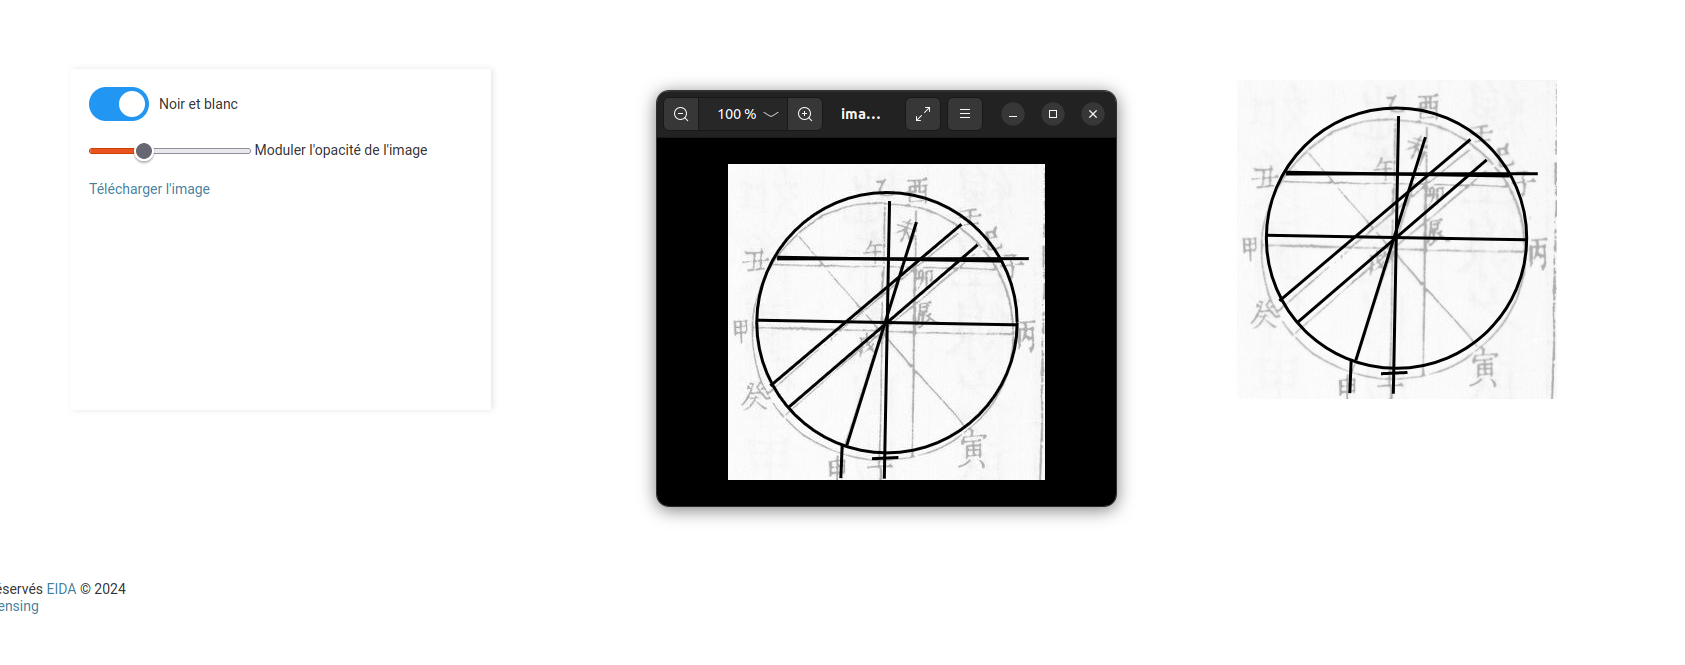
\includegraphics[height=7cm]{figues/manip_vecto.png}
	\end{center}
	\caption{Interface de manipulation des fichiers \svgs, avec exemple d'image modifiée téléchargée.}
	\label{fig:manip_vecto} \end{figure}

J'ai pu ainsi approfondir mes connaissances en JavaScript et découvrir les spécificités du format \svg. La stratégie a consisté à écrire le contenu des fichiers dans le \dom et ajouter de l'interaction grâce à du JavaScript. 

\begin{lstlisting}[language=HTML5, frame=single, breaklines=true, caption={\textit{Template} \html pour la manipulation des fichiers \svgs.}]





{{ regions }}


    {{ block.super }}
    <link rel="stylesheet" href="">
    <link rel="stylesheet" href="">
    <link href="https://cdn.jsdelivr.net/npm/bootstrap-icons@1.8.0/font/bootstrap-icons.css" rel="stylesheet">




    <div class="toolbar">
        <div class="title">
            <b>{{ regions|capfirst }} | page {{ canvas_nb }}</b>
        </div>
    </div>



<div class="container">
    <div class="sidebar">
        <div class="switch-container">
            <label class="switch">
                <input type="checkbox" id="change-stroke-color">
                <span class="slider round"></span>
            </label>
            <label for="change-stroke-color">All lines in blackNoir et blanc</label>
        </div>

        <div>
            <input type="range" min="0" max="1" step="0.01" value="1" id="opacityRange">
            <label for="opacityRange">Toggle Image OpacityModuler l'opacité de l'image</label>
        </div>

        <div>
            <a id="downloadLink" href="#" download="image.jpg">Télécharger l'image</a>
        </div>
    </div>

    <div class="image-container">
        {{ svg_content|safe }}
    </div>
</div>


<script>
    document.addEventListener('DOMContentLoaded', function() {

        const svgElement = document.querySelector('svg'); // Sélectionner l'élément SVG
        const imageElement = document.querySelector('svg image');

        // Charger l'image de fond
        function fond() {
            
            const backgroundImage = "{{ img_file|img_to_iiif:small }}";
            
            imageElement.setAttribute('xlink:href', backgroundImage);
        }
        fond();

        // Changer la couleur des traits
        var toggleSwitch = document.getElementById('change-stroke-color');
        var elementsWithStroke = document.querySelectorAll('[stroke]');
        var originalStrokeColors = [];

        elementsWithStroke.forEach(function(element) {
            originalStrokeColors.push(element.getAttribute('stroke'));
        });

        function changeStrokeColorToBlack() {
            elementsWithStroke.forEach(function(element) {
                element.setAttribute('stroke', 'black');
            });
        }

        function restoreOriginalStrokeColors() {
            elementsWithStroke.forEach(function(element, index) {
                element.setAttribute('stroke', originalStrokeColors[index]);
            });
        }

        toggleSwitch.addEventListener('change', function() {
            if (this.checked) {
                changeStrokeColorToBlack();
            } else {
                restoreOriginalStrokeColors();
            }
        });

        // Modifier l'opacité de l'image
        const opacityRange = document.getElementById("opacityRange");
        opacityRange.addEventListener("input", function() {
            const opacityValue = this.value;
            imageElement.style.opacity = opacityValue;
        });

        // Faire disparaître les éléments onclick
        function removeElementOnClick(event) {
            event.target.remove();
        }

        const circles = document.querySelectorAll('svg circle');
        const paths = document.querySelectorAll('svg path');

        circles.forEach(circle => {
            circle.addEventListener('click', removeElementOnClick);
        });

        paths.forEach(path => {
            path.addEventListener('click', removeElementOnClick);
        });

    // Convertir le SVG modifié en image (PNG ou JPEG)
    function convertModifiedSVGToImage(format, quality, callback) {
        // Sérialiser le SVG modifié
        const svgString = new XMLSerializer().serializeToString(svgElement);

        // Créer un canvas pour dessiner l'image
        const canvas = document.createElement('canvas');
        const context = canvas.getContext('2d');

        // Charger l'image de fond dans le canvas
        const image = new Image();
        image.setAttribute('crossOrigin', 'anonymous');
        image.onload = function() {
            // Le canvas a la même taille que l'image
            canvas.width = image.width;
            canvas.height = image.height;

            // Remplir le canvas avec un fond blanc
            context.fillStyle = 'white';
            context.fillRect(0, 0, canvas.width, canvas.height);

            // Appliquer l'opacité de l'image de fond
            const imageOpacity = parseFloat(window.getComputedStyle(imageElement).opacity);
            context.globalAlpha = isNaN(imageOpacity)~? 1.0~: imageOpacity;
            context.drawImage(image, 0, 0, canvas.width, canvas.height);

            // Réinitialiser l'opacité pour tracer le SVG
            context.globalAlpha = 1.0;

            // Dessiner le SVG modifié sur le canvas
            const svgBlob = new Blob([svgString], { type: 'image/svg+xml;charset=utf-8' });
            const DOMURL = window.URL || window.webkitURL || window;
            const svgUrl = DOMURL.createObjectURL(svgBlob);

            const svgImage = new Image();
            svgImage.onload = function() {
                // Dessiner le SVG à la bonne taille
                context.drawImage(svgImage, 0, 0, canvas.width, canvas.height);

                // Télécharger l'image convertie au format spécifié
                const dataUrl = canvas.toDataURL(`image/${format}`, quality);
                callback(dataUrl); // Utiliser le callback pour manipuler le dataUrl
            };
            svgImage.src = svgUrl;
        };
        image.src = imageElement.getAttribute('xlink:href');
    }

    // Fonction de téléchargement
    function downloadImage(format, quality) {
        convertModifiedSVGToImage(format, quality, function(dataUrl) {
            const downloadLink = document.createElement('a');
            downloadLink.href = dataUrl;
            downloadLink.setAttribute('download', `image.${format}`);
            document.body.appendChild(downloadLink);
            downloadLink.click();
            document.body.removeChild(downloadLink);
        });
    }

    // Lien pour télécharger en JPEG
    const downloadLink = document.getElementById('downloadLink');
    downloadLink.addEventListener('click', function(event) {
        event.preventDefault();
        downloadImage('jpeg', 0.8);
    });

    });
    </script>




\end{lstlisting}

Cette interface est associée à une vue qui renvoie au \textit{template} les informations nécessaires, notamment le contenu du fichier \svg. 

\begin{lstlisting}[language=python, frame=single, breaklines=true, caption={Vue pour relier les données à leur affichage dans l'interface de manipulation.}]
@login_required
def show_crop_vectorization(request, img_file, coords, regions, canvas_nb):
    svg_filename = f"{jpg_to_none(img_file)}_{coords}.svg"
    svg_path = os.path.join(SVG_PATH, svg_filename)

    if not os.path.exists(svg_path):
        print(f"File {svg_path} not found")

    with open(svg_path, "r", encoding="utf-8") as file:
        svg_content = file.read()

    return render(
        request,
        "crop_vecto.html",
        context={
            "img_file": img_file,
            "coords": coords,
            "svg_content": svg_content,
            "regions": regions,
            "canvas_nb": canvas_nb,
        },
    )
\end{lstlisting}

\section{Nouvelles interfaces}

Avec la refonte des interfaces effectuée par les développeuses du projet, ces codes ne sont actuellement plus utilisés dans l'application \aikon, l'utilisation d'un \textit{framework front-end} ayant totalement changé les logiques d'affichage. J'ai cependant eu l'opportunité de poser fondations de la page d'accueil de la plateforme (Fig. \ref{fig:acceuil})~: 

	\begin{figure}[H]
	\begin{center}
		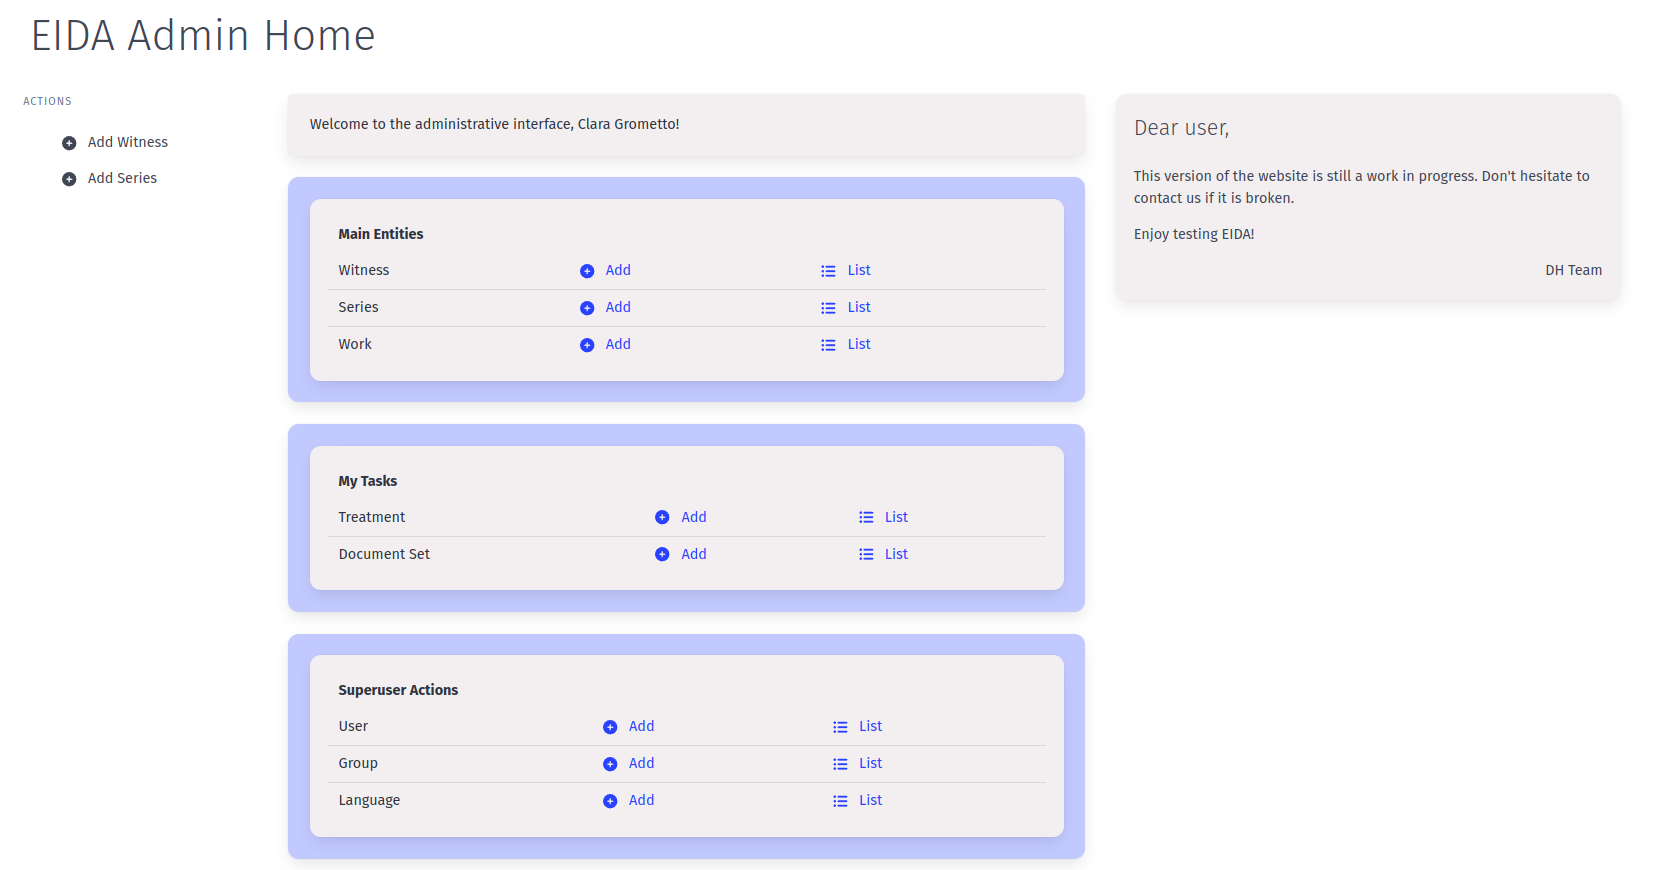
\includegraphics[height=8cm]{figues/accueil.png}
	\end{center}
	\caption{Page d'accueil de la plateforme \aikon}
	\label{fig:accueil} \end{figure}